%!TEX root = Abschluss-ML-Prak-2015.tex
\section{Unser Ansatz}

\begin{frame}{Klassifikation - Sliding Window}
\begin{minipage}{0.59\textwidth}
\begin{itemize}
\item Klassifiziere mittigen Pixel der Eingabe \\
\item Laufe über das Bild (Sliding Window) \\
\item Überspringe Pixel zur Beschleunigung
\end{itemize}
\end{minipage}
\begin{minipage}{0.39\textwidth}
	\flushright
      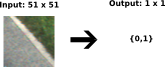
\includegraphics[]{../images/models/sliding_window.png}
\end{minipage}


\visible<2->{
	 \begin{center}
	 \only<1-2> {
        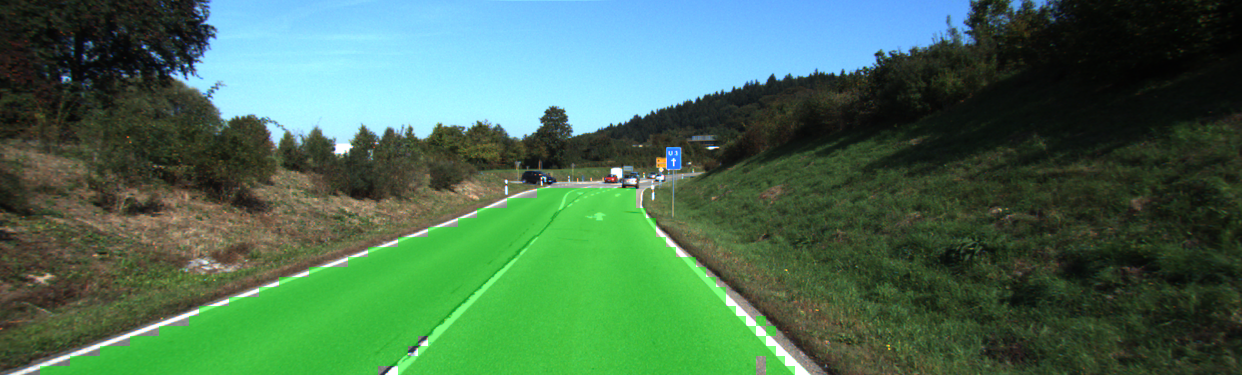
\includegraphics[scale=0.25]{../images/models/stride10.png}
      }
	 \only<3> {
        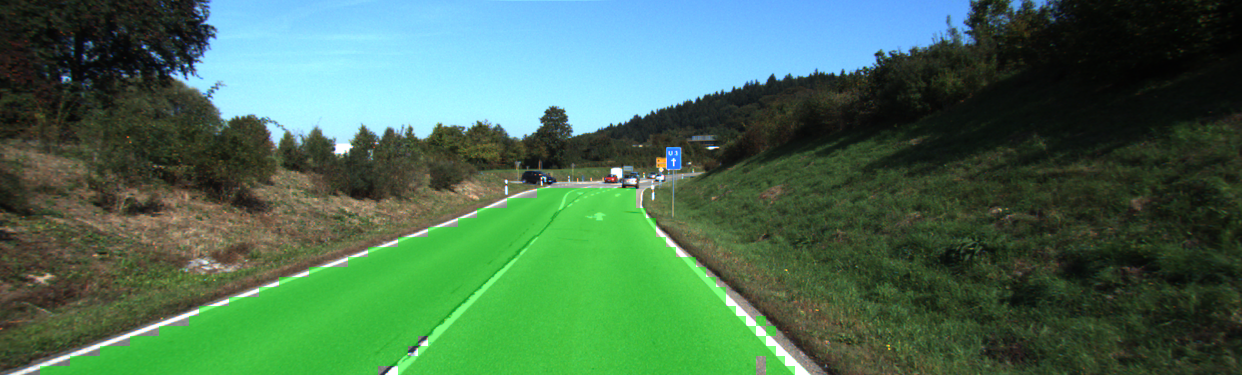
\includegraphics[scale=0.25]{../images/models/stride10.png}
      }
     \end{center}
     }
\end{frame}

\begin{frame}{Regression - Fully - Patch Evaluation}
\begin{minipage}{0.59\textwidth}
\begin{itemize}
\item Nutze Regression und Mean Squared Error Zielfunktion \\
\item Erhalte Information pro Pixel
\item Füge Bild zusammen \\
\end{itemize}
\end{minipage}
\begin{minipage}{0.39\textwidth}
	\flushright
      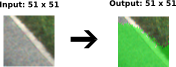
\includegraphics[]{../images/models/fully-conv.png}
\end{minipage}


\visible<2->{
	 \begin{center}
	 \only<1-2> {
        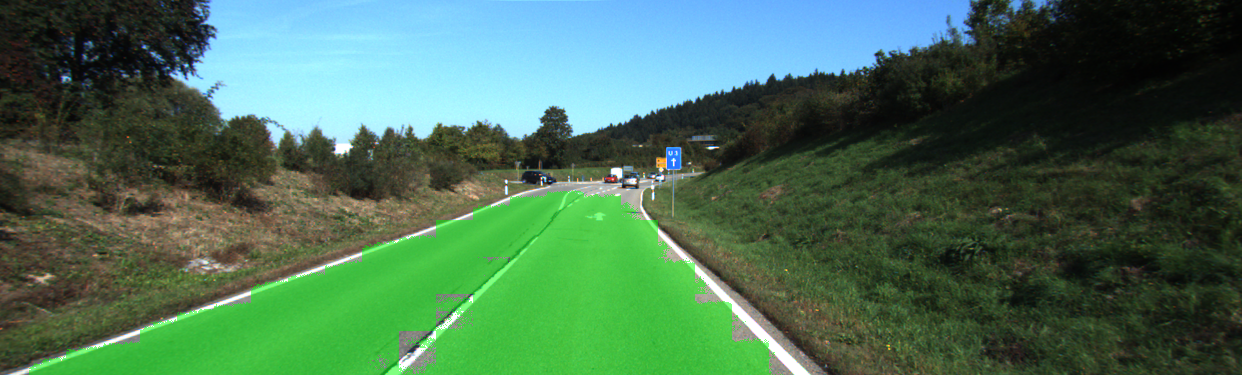
\includegraphics[scale=0.25]{../images/models/fully_stride37.png}
      }
	 \only<3> {
        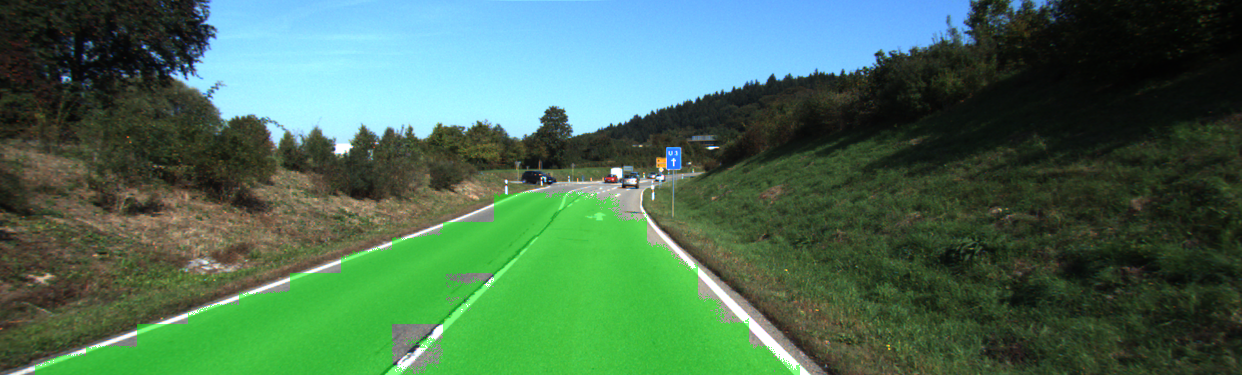
\includegraphics[scale=0.25]{../images/models/fully_stride51.png}
      }
     \end{center}
     }
\end{frame}

\begin{frame}{Aufbau unserer Neuronale Netze}
	\centering
\begin{minipage}{0.49\textwidth}
\centering
Klassifikationsnetz

\begin{itemize}
\item Input Layer $51 \times 51 \times 3$
\item 2 Conv Layer mit \\ 10 Filtern $5 \times 5$
\item 1 Pooling Layer
\item 1 Output Layer $1 \times 1$
\vspace{7em}
\end{itemize}
\end{minipage}
\begin{minipage}{0.49\textwidth}
\centering
Regressionsnetz

\begin{itemize}
\item Input Layer $51 \times 51 \times 3$
\item Hidden Layer mit \\ 10 Filtern $3 \times 3$
\item Pooling Layer
\item Dense Layer
\item Hidden Layer mit \\ 10 Filtern $3 \times 3$
\item Hidden Layer (Deconv) mit \\ 1 Filtern $51 \times 51$
\item 1 Output Layer $1 \times 1$
\end{itemize}

\end{minipage}

\end{frame}